\begin{figure}[!h]
 \centering
\begin{tikzpicture}			
	\node [draw=white, anchor=south west] (label) at (0,0) {
	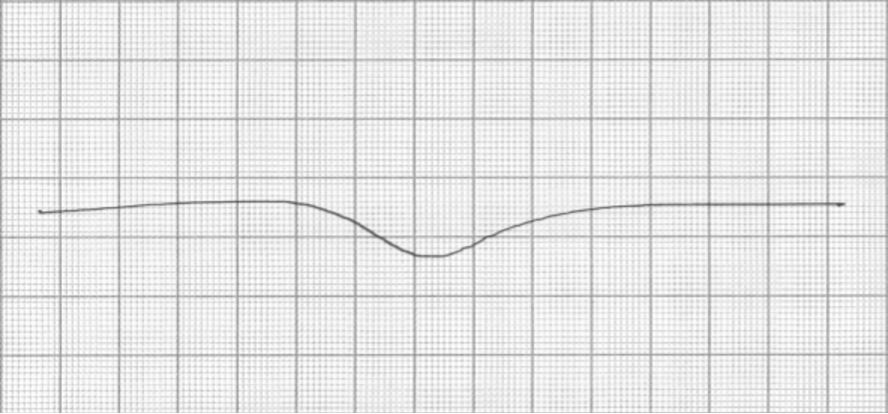
\includegraphics[scale=1]{../Grafiken/Resonanzkurve_15912+_cut.pdf}};
	%\draw (0.15,0.15) circle(0.1) ;
	%\draw[step=.5cm,draw=gray] (0.,0.) grid (\textwidth-10,\textwidth - 240);
	\filldraw (0.8,3.55) circle(0.05) node[above] {$I_{\mathrm{min}}$};
	\filldraw (7.5,2.80) circle(0.05)node[above] {$I_{\mathrm{res}}$};
	\filldraw (14.4,3.7) circle(0.05)node[above] {$I_{\mathrm{max}}$};
	\draw[|-|] (0.8,4.5)--(14.4,4.5) node[midway,above] {$d$};
	\draw[|-|] (0.8,2.5)--(7.5,2.5) node[midway,above] {$d_{res}$};
\end{tikzpicture}
 
 \caption{Beispielhafte Darstellung einer Resonanzkurve für $\SI{15.912}{\mega\hertz}$ mit
 	den eingezeichneten Messpunkten und Abständen, die zur Auswertung genommen wurden. \label{fig:resonanzkurve_20555+_cut}}
 \end{figure} 